\section{Signal quality prediction utilizing Satellite images (v1)}\label{sec:initial_v1}
The system documented in \cite{Thrane2018DriveApproximation} explores the use of colourized satellite images and multiple signal quality metrics as output, e.g. \emph{v1}. The inputs are separated into two neural networks and at a later stage combined into a deep output layer. The inputs and outputs can be observed in Fig. \ref{fig:dnn_architecture_drive_test_minimization}. For this work, the approach was to develop a method that can minimize drive testing, as this is an expensive practice as also highlighted in section \ref{sec:drive_testing}.

\begin{figure}
    \centering
    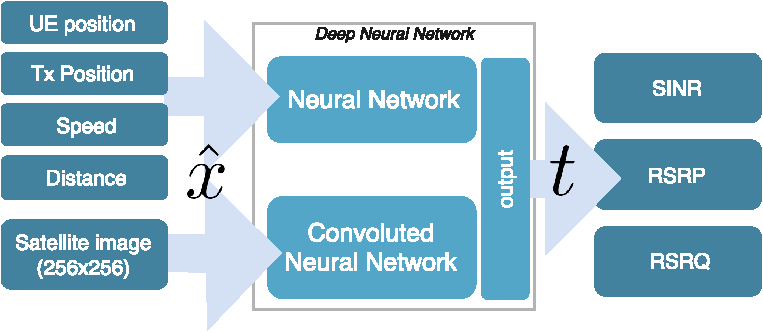
\includegraphics{chapters/part_pathloss/drive_test_minimzation_paper/input_output_figure.pdf}
    \caption{Model architecture used in \cite{Thrane2018DriveApproximation} with a multiple of outputs. Two neural networks are used and concatenated at the output layers.}
    \label{fig:dnn_architecture_drive_test_minimization}
\end{figure}

The size of the layers for both the convolutional neural network and the regular neural network can be seen in Table. \ref{tab:dnn_architecture_drive_test_minimization}

\begin{table}[ht]
  \centering
  \caption{Architecture and layer size of the model used in \cite{Thrane2018DriveApproximation}.}
  \label{tab:dnn_architecture_drive_test_minimization}
  \begin{tabular}{l|l|l}
                & NN settings     & CNN settings      \\ \hline
  Layer size & $[40, 40]$      & $[32, 16, 16, 8]$ \\
  Dropout       & $0.3$           & $0.1$             \\
  Activation    & \textit{ReLU} & \textit{ReLU}  
\end{tabular}
\end{table}

The only regularization added to the model weights were done using dropout layers. The use of dropout layers further enabled so-called \emph{Bayesian approximation} through Monte-Carlo sampling of the layers. The principles are explained in Section \ref{sec:neural_networks}. 

The drive tests detailed in Appendix \ref{app:drive_test_study_2017} compromised the foundation for the data set used for training. The measurements were split into more defined routes as to \emph{emulate} the process of a drive-test and thus limit the available amount of training examples. A total of $39000$ input and target pairs constructed the data set. Of the $\sim 39000$, $\sim 9000$ compromised the test set, as also shown in blue in Fig. \ref{fig:drive_test_routes_split}. Two specified routes, \texttt{Route 1} and \texttt{Route 2}, compose the testing set. Colourized images were used as input to the Deep Learning model. The images were downloaded from Mapbox API \cite{MapboxWebsite}. The colourized images were rotated according to the transmitter to distinguish images at the same position but from different transmitters.

\begin{figure}
    \centering
    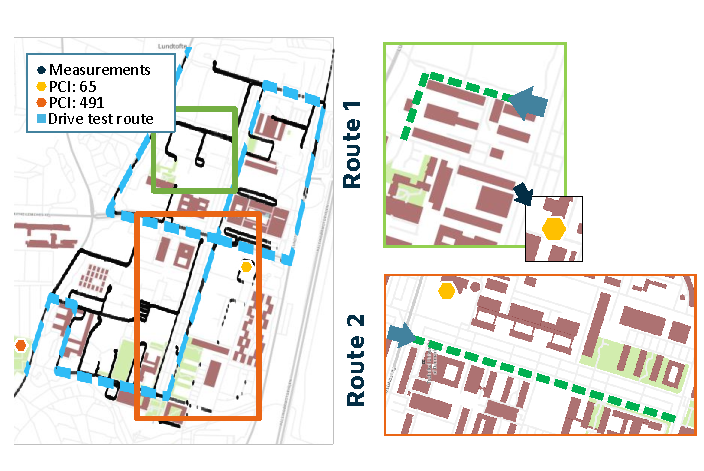
\includegraphics{chapters/part_pathloss/drive_test_minimzation_paper/route_drawing.pdf}
    \caption{The majority of roads at DTU campus area were covered during drive testing. The training was isolated to the main roads of campus, while two specific routes were isolated for testing and evaluation, \texttt{Route 1} and \texttt{Route 2}.}
    \label{fig:drive_test_routes_split}
\end{figure}

The implementation and training of the model was done with open-source libraries \emph{Keras} \cite{chollet2015keras} with \emph{TensorFlow} \cite{tensorflow2015-whitepaper}. The training was accelerated with GPU and mini-batch training. The batch size was heavily limited by the RAM available on the GPU device and was thus limited to $5$. 


\subsection{Results}
\begin{marginfigure}
    \centering
    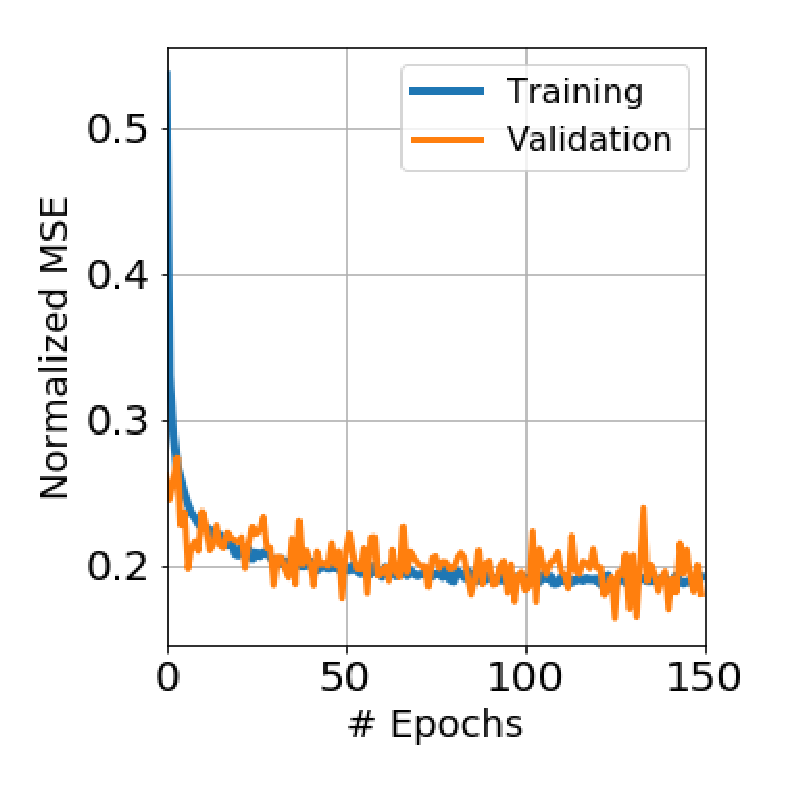
\includegraphics{chapters/part_pathloss/drive_test_minimzation_paper/training_val_test_5ab7fb562d60543b24f857af.eps}
    \caption{Training and validation error for the training of the model.}
    \label{fig:training_val_error}
\end{marginfigure}

The \gls{rmse} error for both rest routes can be observed in Table \ref{tab:rmse_error_v1} for all output metrics. The sampled standard deviation $\sigma$ using the Bayesian approximation method is also presented. The standard deviation can also be presented in terms of a confidence interval, as visualized in Fig. \ref{fig:route_1_v1} (RSRQ as a function of measurement) and \ref{fig:route_2_v1} (RSRP as a function of measurement) along with the prediction (the mean $\mu$) for both rest routes. The measurements are sorted sequentially so the route progression can be studied. This allows for the evaluation of the obstacles during the measurement sequence. For instance, a large obstacle (building) is observed in the radio environment and can be identified by the prediction of the model. 

The \gls{rsrp}, as a function of measurements for route 2, is shown in Fig. \ref{fig:route_2_v1}. It can be seen that a significant decrease in \gls{rsrp} is observed for both predictions and measurements. The decrease in \gls{rsrp} is due to the sequence of measurements. The sequence is increased separation between the transmitter and the receiver, i.e. the vehicle moving away from the \gls{enb}. The trained model captures this and provide sufficient predictions of \gls{rsrp} with an added confidence interval. Most of the measurements are within the $95\%$ confidence interval, which illustrates the usefulness of the Bayesian approximation. 

The training and validation error is shown in Fig. \ref{fig:training_val_error}. The final test error performance of the system (in terms of normalized MSE) was observed to be $\mathbf{0.37}$ MSE. 

\def\arraystretch{1.5}
\begin{table}[]
\centering
\begin{tabular}{@{}lll@{}}
\toprule
\textbf{Parameter} & RMSE   & $\pm \sigma$ \\ \midrule
SINR               & $5.2$ dB & $4.1$ dB       \\
RSRP               & $7.7$ dB & $5.9$ dB       \\
RSRQ               & $3.1$ dB & $2.2$ dB       \\ \bottomrule
\end{tabular}
\caption{\gls{rmse} for both rest routes with the sampled $\sigma$ }\label{tab:rmse_error_v1}
\end{table}



\begin{figure}
    \centering
    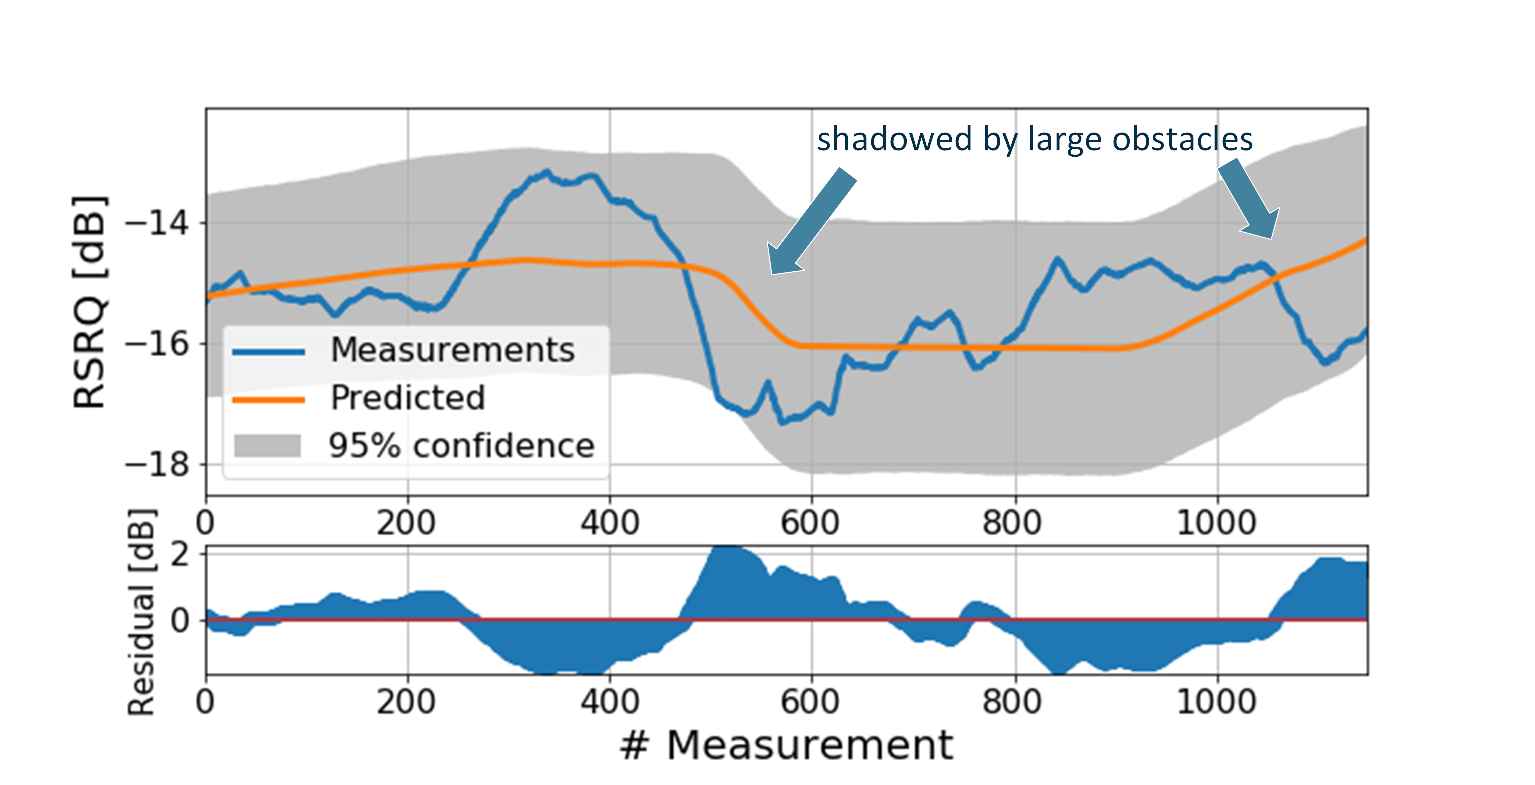
\includegraphics{chapters/part_pathloss/drive_test_minimzation_paper/route_1_predictions_5ab708662d60543b24f857a1_annotated.eps}
    \caption{Prediction of \texttt{route 1} \gls{rsrq} with added $95\%$ confidence interval.}
    \label{fig:route_1_v1}
\end{figure}


\begin{figure}
    \centering
    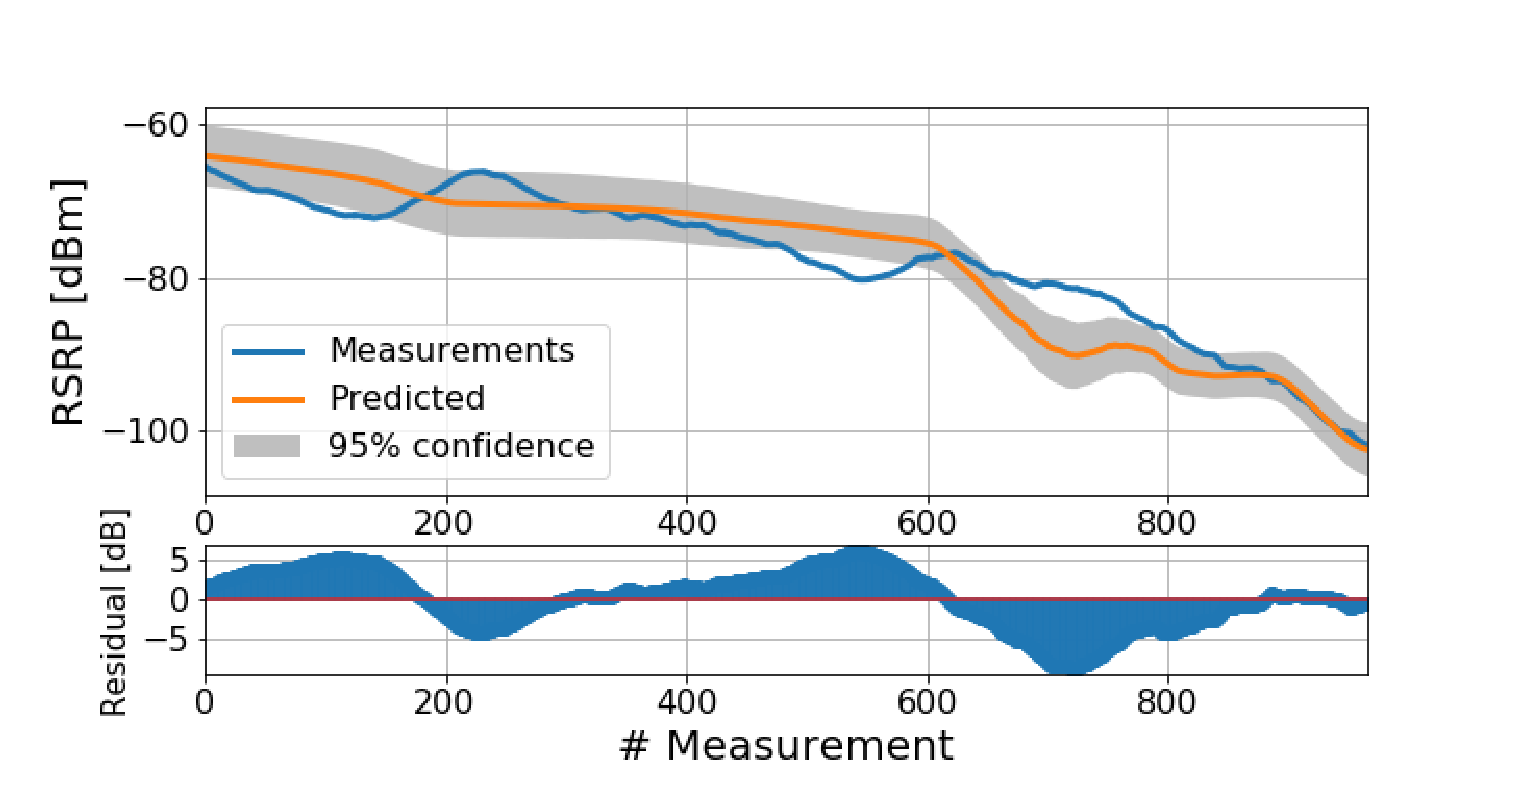
\includegraphics{chapters/part_pathloss/drive_test_minimzation_paper/route_2_predictions_5ab708662d60543b24f857a1.eps}
    \caption{Prediction of \texttt{route 2} \gls{rsrp} with added $95\%$ confidence interval.}
    \label{fig:route_2_v1}
\end{figure}

\subsection{Discussion and Conclusion}
It has been shown that the trained model is capable of providing accurate predictions in unseen areas using limited training data. This was evaluated using two independent routes for testing, e.g. \texttt{route 1} and \texttt{route 2}. From the prediction results of \texttt{route 1}, it was observed that the model is capable of achieving some insight into the local variability. However, it is unknown if the images or sufficient information causes this insight through distance features. It does indicate that the satellite images are useful; however, it requires further studies. 
For \texttt{route 2}, the model is observed to be capable of providing a decrease in \gls{rsrp}, which is primarily related to transmitter and receiver separation distance. 

In terms of model generalization, some issues exist. This is highlighted by the gap between training/validation and test error; thus, further model regularization can improve the overall prediction accuracy of the system. In summary, the \emph{version 1} of utilizing satellite images provided the following conclusion

\begin{itemize}
    \item The model is capable of predicting a drop in \gls{rsrq} explained by the shadowing of a large building.
    \item The model is capable of predicting an accurate decrease in \gls{rsrp} as a function of transmitter-receiver antenna separation.
    \item The gap between training and test error highlights generalization issues
\end{itemize}

It is thus of interest to explore 1) the specific prediction improvements caused by images and 2) the generalization of the model (and techniques hereof)

\section{Generalization issues}\label{sec:summary_version1}
The method has some shortcomings, especially related to generalization. The gap between the test and training set is seen as being significant. However, and possibly most interesting, the documented work introduces the novel idea of introducing automatized meta-data extraction for use in path loss estimation.
As recalled by section \ref{sec:generalization}, \glspl{nn} are capable of providing a satisfactory regression solution to path loss prediction. It is possible and likely that the majority of the accurate path loss predictions are directly related to the primary feature \emph{distance}. The results show that some large-scale fading impairments can be predicted; however, it is unknown if this is due to image-related features. Further studies were deemed a necessity. Specifically, a benchmarking study against traditional path loss prediction methodologies would identify and quantify both the shortcomings and benefits of the documented method. Additionally, it is of interest to study the specific performance gain offered by the inclusion of images. Such a study was completed and published in \cite{Thrane020ModelAidedDeepLearning}.  